\subsection{Voltage measurement}
\label{sec:method_voltage}

\subsubsection{Idea}
Since we are using the internal ADC of the ATMEGA328P microcontroller, which has only a 10-bit ADC, we decided that it would be a good idea to try and make multiple ranges.
That is to make the most of the available resources.
We chose to make two ranges 0-5V and 5-20V. The range switch is performed automatically by the analog circuitry, not the MCU.

\subsubsection{Development}
During development, we faced many issues. Our initial attempts were made with TL072 OP-AMPs since they were in the university parts bin. However due to them not being a rail-to-rail variant, the output voltage couldn't go as low as we wanted it to go without a split rail power supply. 

After proper OP-AMPs arrived we got around to testing our design. After wiring the circuit it seemed to behave sporadically and not as intended. It appeared as if the OP-AMPs worked as an inverter when supplied with a 0V signal. Some forum posts suggested that it may be related to common mode rejection. However, later we found that the problem lied with the power supplies in the Mechatronics Lab. The output of the power supply began to oscillate with 2.5$V_{pp}$ after random amount time of operation. The solution is to just restart the power supply, either by turning it on and off or by turning the current limit to zero and back to some non-zero value. After testing the circuit with a working power supply the circuit worked flawlessly. 

Initially, the switching point was referenced with a zener diode. However, after assembling the first PCB, we found that the 4.8V zener supplied with 5V had a much lower voltage than expected thus we removed it and referenced the switching point to 5V. We could do that since the switching points' stability is not that important.

\subsubsection{Final Implementation}
In the beginning, the initial voltage is divided by four and buffered to not disturb it. The output of the buffer also creates a high range of the voltage measurement section. The schematic of which is shown in Figure \ref{fig:voltageSectionInput}.

\begin{figure}[h]
    \centering
    \frame{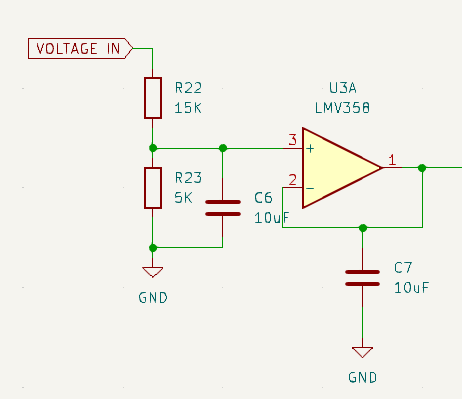
\includegraphics[width=0.5\linewidth]{images/voltageSectionInput.png}}
    \caption{The divider and buffer}
    \label{fig:voltageSectionInput}
\end{figure}

To get the lower voltage range, that is 0-5V, we applied a times four multiplier. That is to reverse the by-four division done by the voltage divider previously. Its schematic is presented in Figure \ref{fig:voltageSectionAmp}.

\begin{figure}[h]
    \centering
    \frame{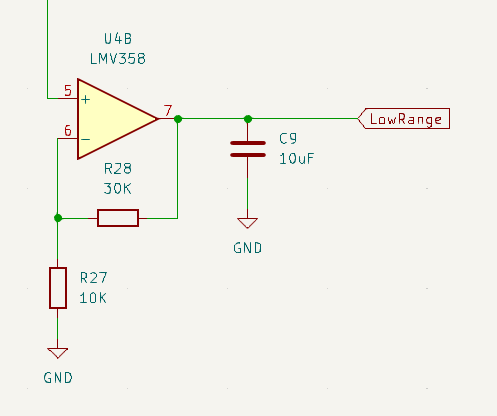
\includegraphics[width=0.5\linewidth]{images/voltageSectionAmp.png}}
    \caption{Lower range amplifier}
    \label{fig:voltageSectionAmp}
\end{figure}

Another part of the voltage section is the comparator which is responsible for detecting the point at which we switch between the different ranges. As we can see in Figure \ref{fig:voltageSectionComp} the comparator is made using the comparator configuration for an OP-AMP. The reference voltage doesn't have to be very stable since it just determines the switching point. The voltage at the inverting input is calculated using the following formula. $$V_{inv}=\frac{V_{ref}}{4}$$ The division is to compensate the initial division that scales the 0-20V to 0-5V.

\begin{figure}[h]
    \centering
    \frame{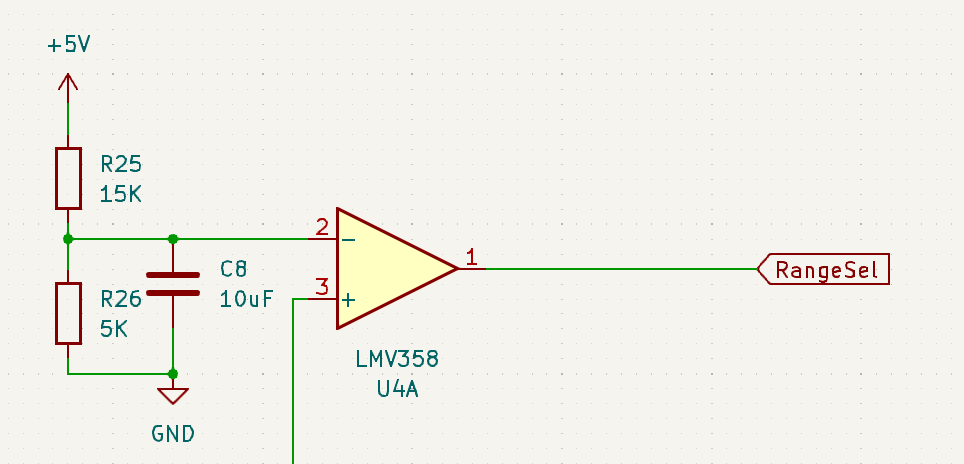
\includegraphics[width=0.5\linewidth]{images/voltageSectionComp.png}}
    \caption{Range select comparator}
    \label{fig:voltageSectionComp}
\end{figure}

The range switching itself is done by the use of a signal relay. To drive the relay we use a standard NMOS transistor. The circuitry can be seen in Figure \ref{fig:voltageSectionRelay}. The relay switches between the direct output of the buffer and the amplifier which are presented in Figure \ref{fig:voltageSectionInput} and Figure \ref{fig:voltageSectionAmp} respectively.

\begin{figure}[h]
    \centering
    \frame{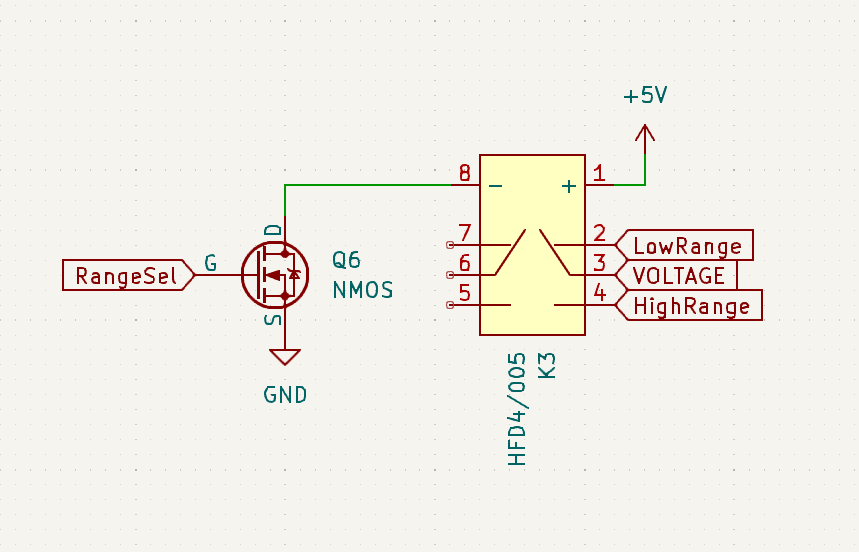
\includegraphics[width=0.5\linewidth]{images/voltageSectionRelay.png}}
    \caption{Range switching relay}
    \label{fig:voltageSectionRelay}
\end{figure}

The relay is controlled by the signal from the comparator. However, this signal also tells the microcontroller what range has been selected by the analog front end. The full circuit can be seen in the schematic, block 14. in section \ref{sec:appendix}.
\FloatBarrier